\documentclass{standalone}
\usepackage{tikz}
\tikzset{block/.style = {draw, fill=white, very thick, rectangle, minimum height=1cm, minimum width=2cm},  
         square/.style = {draw, fill=white, very thick, rectangle, minimum height=1cm, minimum width=1cm},
         sum/.style= {draw, fill=white, very thick, circle, node distance=0.5cm}}  
\begin{document}
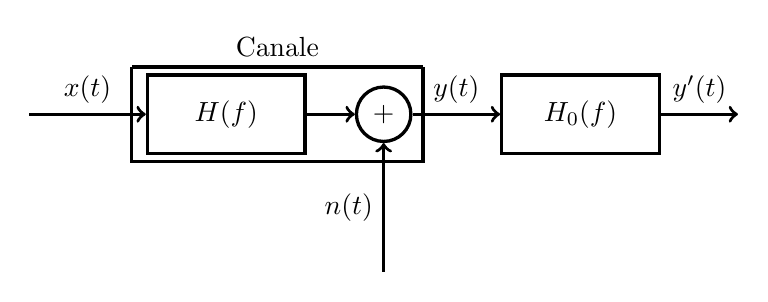
\begin{tikzpicture}[scale=2]
    \node[sum](h)at(0.25,0){+};
    \node[block](+)at(-0.75,0){$H(f)$};
    \draw[very thick,->](-2,0)--(+.180)node[midway, above]{$x(t)$};
    \draw[very thick,->](0.25,-1)--(h.270)node[midway, left]{$n(t)$};
    \draw[very thick,->](+.0)--(h.180);
    \node[block](adc)at(1.5,0){$H_0(f)$};
    %\node[block](s)at(3,0){};
    \draw[very thick,->](h.0)--(adc.180)node[midway, above]{$y(t)$};
    \draw[very thick,->](adc.0)--(2.5,0)node[midway, above]{$y'(t)$};
    %\draw[very thick,->](adc.0)--(s.180);
    %\draw[very thick,->](s.0)--(4,0);
    %\draw(1.25,0)--(1.365,0)--(1.625,0.175);
    %\draw(1.625,0)--(1.75,0);
    %\draw(2.75,-0.175)--(3,-0.175)--(3,0.175)--(3.25,0.175);
    %\draw[very thick](2.875,0)--(3.125,0);

    \draw[very thick](-1.35,0.3)--(-1.35,-0.3)--(0.5,-0.3)--(0.5,0.3);
    \draw[very thick](0.5,0.3)--(-1.35,0.3)node[midway, above]{Canale};
\end{tikzpicture}
\end{document}